\documentclass{ba-kecs}
\usepackage{graphicx}
\usepackage[]{algorithmicx}
\usepackage{algpseudocode}
\usepackage{algorithm}
\usepackage{amsmath}




\title{AI implementations for Hex}
\runningtitle{AI for Hex}

\author{A. Steckelberg, N. Vaessen, J.L. Velasquez, J. Vermazeren, T. Wall, X. Weber}

\begin{document}

\maketitle

\begin{abstract}
 Hex is a classic board game invented in 1942 by Piet Hein and independently by John Nash in 1948. In this paper there is research into alpha-beta  and Monte Carlo Tree Search Hex players. We compare different evaluation functions which includes Dijkstra, Electric Circuit besides this we compare Monte Carlo Tree Search specific heuristics.   
\end{abstract}

\section{Introduction}
Hex is a well-known board game first created in 1942 by Piet Hein, a Danish physicist, with later improvements being made by John F. Nash in 1948. It gained the name Hex in 1952 when a version of the game was release by the firm Parker Brothers, Inc \cite{gardener1959hex}. The basic idea of Hex is to create a bridge across a diamond shape board of hexagons. The generally accepted normal size of the board is 11 $\times$ 11, however it can be played on boards of differing sizes. One player will try to create a bridge from the top of the board to the bottom, while the other player tries to make one from left to right. The game is fully deterministic, as by finishing one player’s bridge will always block the other player. As the first player is always at an advantage, Hex has a unique rule to address this. Called the Pie Rule, it states that after the second player has had their first move, they may switch the placement of the first two tiles.

The history of creating algorithms to play Hex is rich with successful attempts, all using a different approach. In this report, several of these attempts will be implemented and tested against both each other, while also seeing if limiting factors in these algorithms (time per move, tree depth, etc.) have major effects on the results.



\section{Rules and Algorithms of Hex}
\subsection{Rules}
Rules for Hex
\subsection{Alpha-beta Hex Players}
The alpha-beta player consists of a player which uses a minimax game tree and applies $\alpha - \beta$ pruning as it builds the tree.
% cite Artificial Intelligence: A Modern approach
\subsubsection{Minimax algorithm}
The minimax algorithm tries to find the best next possible action by fully expanding each node and seeing all possible moves in a certain depth. After the tree is fully expanded the leaf nodes are evaluated and given a value. 

\subsection{Electric circuit}
Explanation of the electric circuit of Anshelivic

\subsection{Monte Carlo Tree Search}
A powerful A.I. technique for board games is the Monte Carlo Tree Search(MCTS). It applies optimization techniques of random simulations to the game tree. 

The game tree closely follows a \textit{Markov Decision Process} (MDP) in which every node of the tree is represented by a State $s \in S$ and the connection between the nodes is represented by an action $a \in A$.
\begin{itemize}
\item $S$: a set of all possible states of the board
\item $A$: a set of all possible actions that can transition from one state to the other
\item $P_a(s, s')$: the probability of reaching state $s'$ by using action $a$ on state $s$
\item $R_a(s, s')$: the reward for reaching state $s'$ by using action $a$ on state $s$
\end{itemize}

For Hex, the probability of reaching a state for any action is 1 as long as it is a legal move. 
\begin{figure}
	\centering
	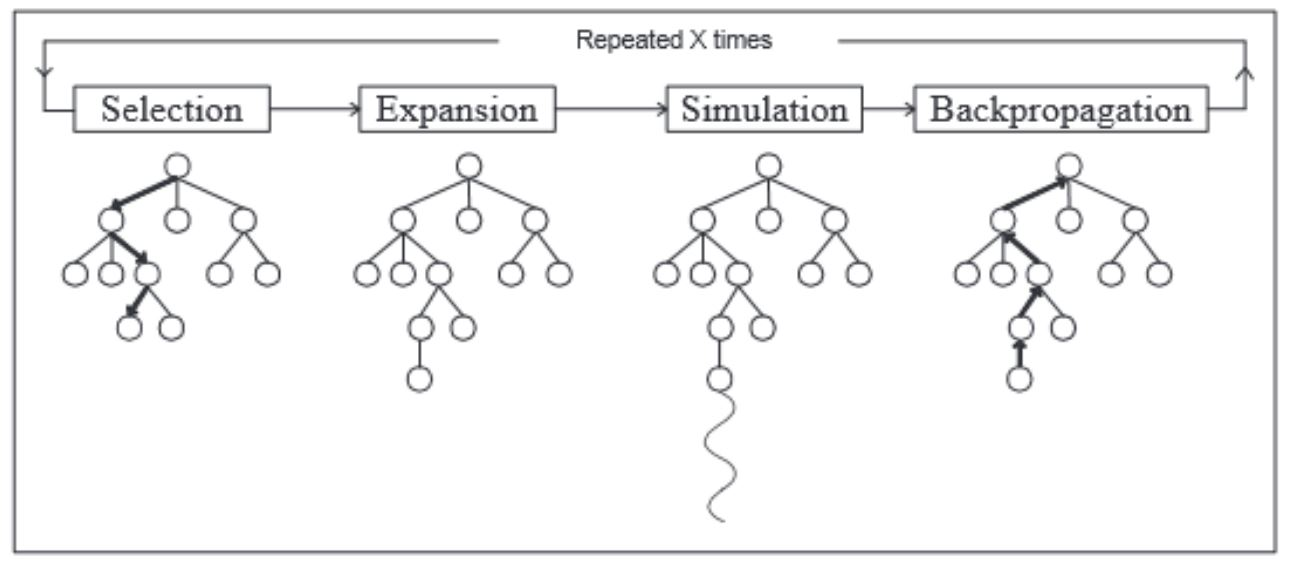
\includegraphics[width=0.5\textwidth]{figure_mcts.jpg}
	\caption{The four steps of Monte-Carlo Tree Search \cite{chaslot2008progressive}}
	\label{fig:mcts}
	\end{figure}
The MCTS algorithm can be divided into four main parts(see figure \ref{fig:mcts}): 
\begin{enumerate}
\item Selection: In this part the algorithm looks for the most urgent node with a state $s$ that hasn't being visited before.
\item Expansion: one or more nodes are expanded by adding leaf nodes according the values left in $A$.
\item Simulation: a simulation takes place in order to assign a reward value to the newly added node/s.
\item Backpropagation: the statistics of the tree are updated through backpropagation.
\end{enumerate}

These four simple parts of the algorithm can be divided into two policies that simplify the process.
\begin{itemize}
\item \textit{Tree Policy}: in this policy the stages of selection and expansion take place. The random nodes are selected and expanded, ready to receive their reward value.
\item \textit{Default Policy}: in this policy the simulation takes place and a reward value is given to the node 
\end{itemize}
The backpropagation stage of the MCTS does not occur within any policy as it just represents the update of the tree after the reward, which is used in later cycles for the tree policy to select and expand new nodes.



\begin{algorithm}
    \caption{Monte-Carlo Tree Search}
    \label{MCTS}
    \begin{algorithmic}
        \Procedure{MCTS}{$s_0$} 
            \State create root node $v_0$ with state $s_0$
            \While{within computational budget} 
                \State $v_l \gets$ TreePolicy($v_0$)
                \State $ \Delta \gets$ DefaultPolicy($s(v_l)$)
                \State Backup($v_l, \Delta$)
            \EndWhile\label{}
            \State \textbf{return} $a$(BestChild($v_0$))
        \EndProcedure
    \end{algorithmic}
\end{algorithm}

In Algorithm 1 we see the general structure of the MCTS. The root of the tree will be the board state at the beginning current turn. After the tree has fully expanded according to computational budget using the repeated MCTS process explained before, the best child is selected. We return the action $a$ which connects the current state $s$ to the best child.
\subsection{Improvements on General MCTS}
Different heuristics can be used on top the MCTS algorithm to enhance its performance.
\subsubsection{Upper Confidence Bounds for Trees (UCT)}
%%reference Peter Auer
The UCT is an algorithm which adapts the Upper Confidence Bounds (UCB) exploitation and exploration of trade-offs as a tree policy. 
Selecting a child node to traverse in the selection part of MCTS can be seen as a multi-armed bandit problem.
The UCT tree policy works by choosing the node $v$ that maximizes the independent multi-armed bandit problem:
\begin{center}
\begin{equation}
	UCT = \bar{X_v} + C_p \sqrt{\frac{\ln n}{n_v}}
\end{equation}
\end{center}
In the equation above $n$ represents the amount of time the current node has being visited,$n_v$ the amount of time a  child node has been visited, and the constant $C_p >=0 $ can be used to weight the importance of exploration. If a child is not visited ($n_v = 0$) the exploration term is set to $\infty$.

\begin{algorithm}
	\caption{Upper Confidence Threshold}
    \label{UCT}
    \begin{algorithmic}
    	\Function{UCTSearch}{$s_0$}
        	\State $v_0 \leftarrow$ create root node from $s_0$
            \While{within computational budget}
            	\State $v_l \leftarrow$ TreePolicy($v_0$)
                \State $\Delta \leftarrow$ DefaultPolicy($s(v_l)$)
                \State Backup($v_0, \Delta$)
            \EndWhile
            \State \textbf{return} $a$(BestChild($v_0,0$))
        \EndFunction
        \State
        \Function{TreePolicy}{$v$}
        	\While{$v$ is non-terminal}
            	\If{$v$ not fully expanded}
                	\State \textbf{return} Expand($v$)
                \Else
                	\State $v \leftarrow$ BestChild($v_0,Cp$)
                \EndIf
            \EndWhile
           	\State \textbf{return} $v$
        \EndFunction
        \State
        \Function{Expand}{$v$}
        	\State $a\leftarrow$ any random unused action in $A(s(v))$
            \State add new child $v'$ to $v$ where:
            \State $s(v') =$ Result($s(v),a$)
            \State $a = a(v')$
            \State \textbf{return} $v'$
        \EndFunction
        \State
        \Function{BestChild}{$v,c$}
        	\State \textbf{return} $\operatornamewithlimits{arg max}\limits_{v' \in children(v)}\frac{Q(v'))}{N(v')} + c\sqrt{\frac{\ln N(v)}{N(v')}}
$
        \EndFunction
        \State
        \Function{DefaultPolicy}{$s$}
        	\While{$s$ is non-terminal}
            	\State choose $a \in A(s)$ uniformly at random
                \State $s \leftarrow$ Result($s, a$)
                \State \textbf{return} reward for state $a$
            \EndWhile
        \EndFunction
        \State
        \Function{Backup}{$v, \Delta$}
        	\While{$v$ is not null}
            	\State $N(v) \leftarrow N(v)+1$
                \State $Q(v) \leftarrow Q(v)+\Delta(v,p)$
                \State $v \leftarrow$ parent of $v$
            \EndWhile
        \EndFunction
    \end{algorithmic}
\end{algorithm}

\subsubsection{AMAF}
Originally the AMAF method has been introduced to improve the learning process inside MCTS trees. The selection of the UCT algorithm is based on a estimated value obtained by simulating the move in the node a couple times. This can lead to a problem if there is a large state space since the algorithm has to do many simulations before it can sample all the moves in a node. To conquer this issue AMAF, also known as RAVE, is introduced.\\
\\
For every node the algorithm stores for all legal moves the following values 
\begin{itemize}
	\item The average UCT result obtained from all simulations in which move $a$ is performed in state $s$
	\item The average AMAF result, obtained from all the simulations in which move $a$ is performed further down the path that passes by node $s$
\end{itemize}



When backpropagating the result of a simulation in a certain node \textit{t} in the tree, the UCT result is updated for the move $a$ that was directly played in the state, and the AMAF value is updated for all the legal moves in node $t$ that have been encountered at a later stage in the simulations. AMAF will encounter more samples and will use them to make better predictions. However, the disadvantage of this information is that AMAF information is more global whilst the UCT information is more local. This makes AMAF scores useful for less visited nodes, but when the number of visits increases, the UCT values should become more important. \cite{sironicomparison}


To solve this issue the AMAF algorithm keeps track of the two scores separately and uses a weight $\beta$ to reduce the importance of the AMAF score over time. 


\subsubsection{Parallelisation}
There are three different types of parallelisation, depending on in what stage Monto-Carlo Tree Search is parallelised. The three options are: leaf parallelisation, root parallelisation and tree parallelisation. 

In this paper we only consider leaf parallelisation since this is a straightforward to implement. To select a leaf node this method uses one main thread, which is the same thread that runs the game logic. From this leaf node it simulates independent games for each available thread. When all games are finished the main thread backpropagates all the values.\cite{chaslot2008parallel} Leaf parallelisation is depicted in figure \ref{fig:leaf}.

A problem with leaf parallelisation is that threads have to wait for each other which could slow then the process a way to solve this is end simulations for a move if a certain amount of games is won. For instance, if 16 threads are available, and 8 (faster) finished games are all losses, it will be highly probable that most games
will lead to a loss. Therefore, playing 8 more games is a waste of computational power. This will enable the program to traverse the tree more often.\cite{chaslot2008parallel}

To reduce the cost of using threads we implemented both the \textit{Java ExecutorService} interface and \textit{ThreadGroups} and we compared them
\begin{figure}
	\centering
	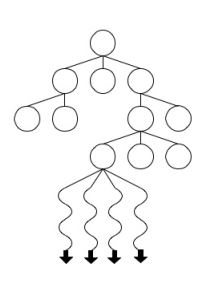
\includegraphics[]{figure_leafparallisation}
		\caption{Visual explanation of leaf parallelisation, the down arrows are the threads \cite{chaslot2008parallel}}
		\label{fig:leaf}
\end{figure}


\subsubsection{Tree reuse}
The ordinary implementation of Monte-Carlo Tree Search builds a new tree for every move a player has to make. An obvious improvement to speed up the algorithm would be that the program does not build a tree every move but it tries to keep the tree it made in the previous move by searching through the children of the previous move and check if the node already exist. Since the program does not know the move of the opponent it could be that the move does not exist This strategy enables the algorithm to have already some reward values for certain moves so the predictions can be done more accurately.

\section{Experiments}
Explanation of experiments and results, comparing different parameters
\section{Results}
Explanation of results of the experiments
\section{Conclusion}
Conclusion on the explanation of the result of the experiments
\bibliography{biblio}



\end{document}

